\paragraph{Tijdsduur}
\begin{figure}[H]
    \centering
    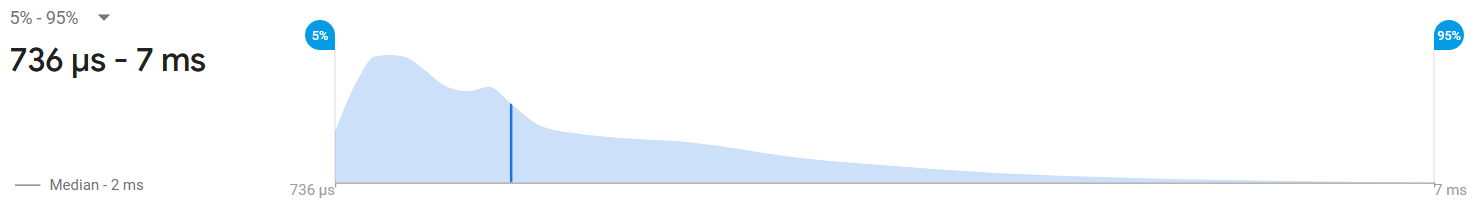
\includegraphics[height=0.085\textheight]{sensorenDuratieNativeAccelerometer.png}
    \caption{Overzicht tijdsduur ophalen van accelerometer data bij Android.}
\end{figure}
Van zodra er op de knop wordt gedrukt om gegevens op te halen van de accelerometer blijft de applicatie
dit continu doen. Hierdoor worden er honderden metingen gedaan die ons vertellen dat het ophalen 
van de accelerometer data gemiddeld 2ms duurt. De minimum en maximum waarden liggen op 736µs en 7ms.
\begin{figure}[H]
    \centering
    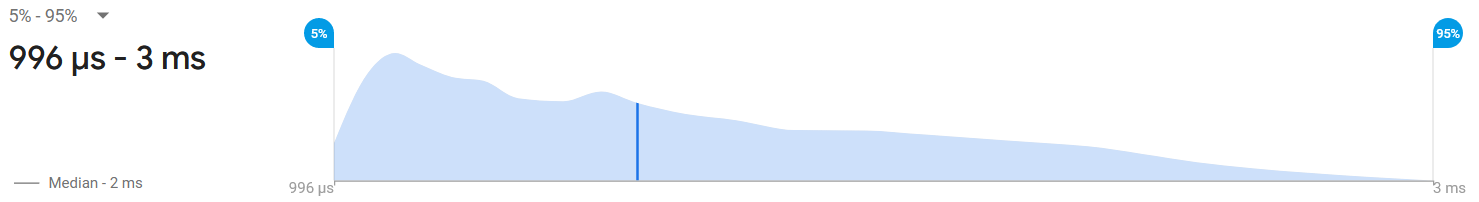
\includegraphics[height=0.085\textheight]{sensorenDuratieNativeGyroscoop.png}
    \caption{Overzicht tijdsduur ophalen van gyroscoop data bij Android.}
\end{figure}
Net zoals bij de accelerometer worden er constant gegevens opgehaald van zodra er op de knop wordt gedrukt. 
Hierdoor worden er opnieuw honderden metingen gedaan die ons vertellen dat het ophalen 
van de gyroscoop data gemiddeld 2ms duurt. De minimum en maximum waarden liggen op 996µs en 3ms.

\paragraph{CPU \& geheugen}
\begin{figure}[H]
    \centering
    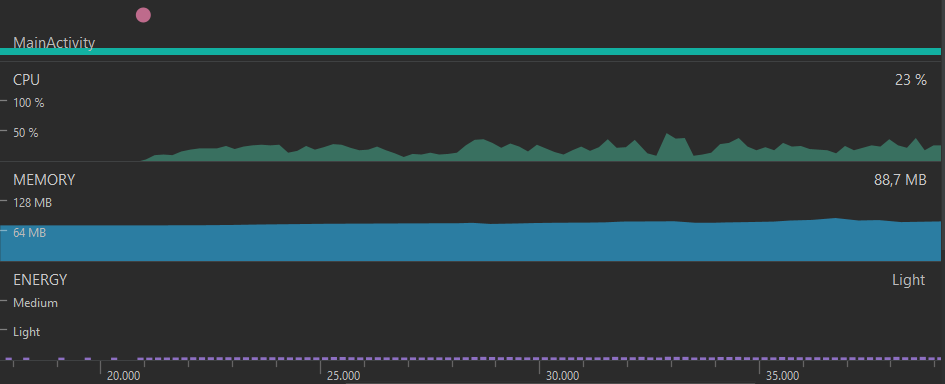
\includegraphics[height=0.25\textheight]{sensorenPerformantieNativeAccelerometer.png}
    \caption{Overzicht CPU en geheugen gebruik tijdens het ophalen van accelerometer data bij Android.}
\end{figure}
Op de grafiek is te zien dat het CPU gebruik van de applicatie bij het ophalen van de accelerometer data,
gemiddeld 23\% is met toch wel redelijke schommelingen. Wanneer er nog geen data wordt opgehaald, wordt de CPU niet 
gebruikt. Het geheugen blijft rond de 88MB hangen, met verschillen van maximum 4-5MB. 
Er is geen merkbaar verschil in het geheugen wanneer er data wordt opgehaald of wanneer er 
geen data wordt opgehaald.
\begin{figure}[H]
    \centering
    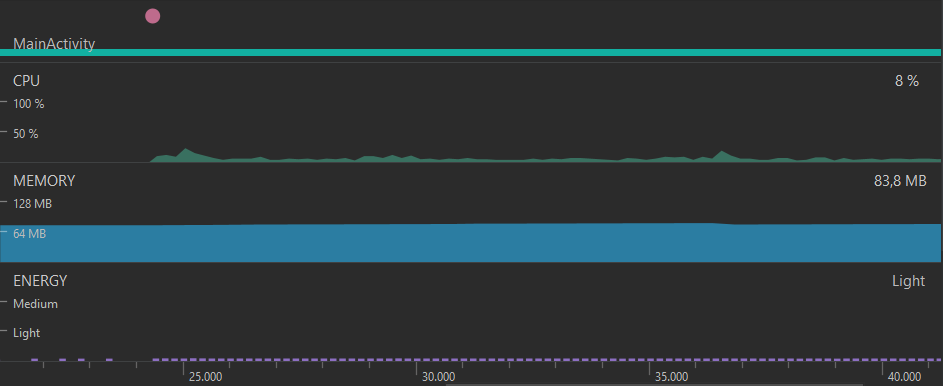
\includegraphics[height=0.25\textheight]{sensorenPerformantieNativeGyroscoop.png}
    \caption{Overzicht CPU en geheugen gebruik tijdens het ophalen van gyroscoop data bij Android.}
\end{figure}
Net zoals bij de accelerometer is op de grafiek te zien dat het CPU gebruik van de applicatie bij het 
ophalen van de gyroscoop data, gemiddeld 8\% is. Wat opvalt, is dat er bij het ophalen van de gyroscoop data
in het begin een piek is van 30\%. Maar dat dit daarna terug zakt naar 8\%. Bij de accelerometer was er geen
piek te zien maar was het gemiddelde CPU gebruik wel hoger. Net zoals bij de accelerometer is er ook geen 
CPU gebruik wanneer er geen data wordt opgehaald. Het geheugen blijft terug rond de 88MB hangen, met 
verschillen van maximum 4-5MB. Opnieuw is er geen merkbaar verschil in het 
geheugen wanneer er data wordt opgehaald of wanneer er geen data wordt opgehaald.
  
